\documentclass[a4paper,12pt]{article}
\usepackage[utf8]{inputenc}
\usepackage[margin=0.5in]{geometry} % Normal Margins
\usepackage{sectsty} % Center sections
\allsectionsfont{\centering}
\usepackage{setspace} % Double Spacing
\doublespacing
\usepackage{hyperref} % URL in bibio
\usepackage{graphicx} % Image
\graphicspath{ {/} }

\title{The Smart Way to Transfer Data in Smart Cities}
\author{Dalton Russell Cole}

\begin{document}

\clearpage\maketitle
\thispagestyle{empty}
\newpage
\clearpage
\setcounter{page}{1}


\section*{Abstract}
\paragraph{}
The future of cities will be Smart Cities. With the popularity that Internet of Things is attracting, smart cities are the next natural step in urban development. In this literature review, \cite{SC} will be discussed. In \cite{SC}, NomaBlue is introduced, which is a new take on spatial recognition in smart cities. The system is based on gathering nomadic data from users in a collaborative fashion using smart Bluetooth technology. The example of sharing shop data is presented, such as discounts and number of people currently in the store. Two case studies were completed, one involving several students at a university and another involving a simulation of 83 years. The stuides concluded that the storing of geo-location data and the transfer of data using Bluetooth is a viable means of mapping out unfamilar locations, however, there is future work to be done. This paper will also discuss the idea of smart cities as presented in \cite{IOT} and their potential uses.

\section*{Internet of Things for Smart Cities}
\paragraph{}
In this section, \cite{IOT} will be discussed. The Internet of Things (IoT) is currently on the rise. The IoT is the use of small devices for various tasks such as collecting data, sending data, relaying, and many more simple tasks that require very little processing power. The IoT has many possible applications, one of which is in smart cities. Within smart cities, IoT could have many different applications, such as: structural health, waste management, air quality, noise monitoring, traffic congestion, city energy consumption, smart parking, smart lighting, and automation and salubrity of public buildings.
\paragraph{}
IoT devices could be placed in buildings to constantly measure structural health. Vibration and deformation sensors could be placed throughout the building to monitor attributes such as building stress. These sensors could be combined with other sensors to get a better understanding of small earthquakes on city buildings. Intelligent waste containers are a possible use of IoT devices in waste management. 
\paragraph{}
The European Union has recently adopted a 20-20-20 Renewable Energy Directive to decrease climate change. The directive calls for a 20\% reduction in greenhouse gas emissions, a 20\% cut in energy consumption, and a 20\% increase in renewable energy by 2020. The first 20 in this initiative is an incentive to use IoT devices for air quality control. Air quality measurement devices can be placed around a smart city to continuously monitor air conditions. With a continuous stream of data, preventative models can be imposed with thorough data down to the second of each day. 
\paragraph{}
Noise monitoring could be imposed with a slew of IoT devices. This monitoring could be used for a number of things, such as keeping noise pollution down through noise level enforcement. Another potential benefit is in the public security realm. The devices could be used to detect noises such as glass crashes or brawls, alerting authorities when either of these sounds are heard. There are obvious privacy risks with the aforementioned use of IoT devices. 
\paragraph{}
Traffic congestion and smart parking are two purposes that the general public will likely get behind to push cities into becoming smart cities. IoT devices could be used throughout roadways and give drivers live updates on traffic conditions, similar to the Waze App \cite{waze}. Smart parking could be utilized by having road sensors along with intelligent displays that are used to direct motorists to empty parking spots. Not only will citizens get behind these two ideas, but environmentalist as well. With the continuous monitoring of traffic and parking, drivers will have to drive a shorter distance to get to their final destination, thus eliminating carbon dioxide emissions.
\paragraph{}
City energy consumption, smart lighting, and the automation and salubrity of public buildings are big environmental applications as well. Power grid monitoring devices could be placed around the city to continuously monitor power usage throughout. Detailed maps could be drawn, seeing what uses the most energy and possible ways that they could cut back on usage. Smart lighting could be deployed on city street lights to increase usage when needed, and decrease usage when not. The lights would be able to monitor weather conditions and have motion detectors, illuminating the streets only when necessary. Automation and salubrity of public buildings has the potential to keep citizens more comfortable by measuring temperature and humidity as well as reducing heating/cooling costs.
\paragraph{}
With the constrained nature of IoT devices, they must be able to handle the load of daily task along with external communication abilities. The IETF standards are a popular base for IoT devices for their open and royalty-free nature. For every protocol stack, there must be a constrained version to be run on IoT devices. For example, HTML/XML has EXI (Efficient XML Interchange), HTTP/TCP has Constrained Application Protocol(CoAp)/UDP, and IPv4/IPv6 has IPv6/6LoWPAN. The size of the HTML and XML messages are too large for highly limited devices to handle. EXI is an alternative to these two in IoT devices. EXI has schema-less and schema-informed encodings. These encodings allow the devices to communicate with outside devices using HTML and XML. The reason why HTTP is so popular is mostly due to its high readability, however, this is a drawback for IoT devices with their limited computing power. HTTP normally relies on the TCP protocol for data transfer, which has costly overhead for these devices. CoAP is one possible solution to these challenges. CoAP proposes a binary format that is transported over UDP. Retransmission is only done when a reliable service is required. CoAP is a great solution because it supports ReST methods, there is a one-to-one mapping between the two protocols, and because it supports a wide range of HTTP use scenarios. 
\paragraph{}
With the large number of IoT devices in a smart city, the network layer becomes an issue as well. Many devices currently uses the IPv4 address space, however, these addresses are running out. IPv6 is the solution to the lack of IPv4 address, but, with the address's large space comes extra overhead. IPv6 uses a 128-bit address field, which can be a costly overhead. 6LoWPAN is an established solution to this overhead that works by compressing the IPv6 and UDP headers in constrained networks. When packets are sent using 6LoWPAN, a boarder router performs a conversion between 6LoWPAN and IPv6 and vice-versa. This creates its own issues however. Many IPv4 devices do not accept traffic from IPv6, so there must be some sort of conversion from IPv6 to IPv4. To overcome this, a Network Address and Port Translation like solution can be implemented. An edge router can map IPv6 addresses to a single IPv4 address in outgoing traffic. Incoming IPv4 traffic can go to a specific port on the edge router that will map the traffic to an IPv6 internal address.
\paragraph{}
This paper conducted a proof-of-concept experimental study in Padova, Italy. In this experiment, an idea similar to the previously mentioned \textit{smart lighting} is implemented. Wireless nodes will be monitoring public street lighting and collecting environmental data. The nodes will be equipped with multiple sensors, such as: photometer, temperature, humidity, and benzene sensors. The IoT devices will be placed on streetlights throughout the city. The photometer sensor is used to measure the intensity of the lamp's light at regular time intervals, or upon request by an administrator. The benzene sensor is used to measure benzene ($C_6H_6$) in the air. 
\paragraph{}
The nodes implement a multi-hop 6LoWPAN cloud that uses IEEE 802.15.4 to transfer data. Each node is given a unique IPv6 address which is then compressed using the 6LoWPAN protocol. A gateway node is required to bring the data from the internal network to the live network. This allows each node to be individually accessible from the Internet.
\paragraph{}
The nodes collected data on: temperature, humidity, light, and benzene. This data can be used to find interesting correlations between these factors among others. One such correlation is decrease benzene levels at night, which is likely due to the decrease in traffic during this time. Surprisingly, there was no variation of benzene levels during the day time, such as would be expected during rush-hour traffic. The highest levels of benzene was experienced on October 29th in the early afternoon. Looking at the data from the other sensors, there was a decrease in light intensity and temperature in addition to an increase in humidity. This points to a quick rainstorm that happened on this day, resulting in peak benzene levels. The data collected from these IoT devices in this proof-of-concept experiment is vital is showing that smart cities can be a valuable asset to future wellbeing and success.

\section*{A novel Bluetooth low energy based system for spatial exploration in smart cities}
\paragraph{}
In this section, the main paper for this literature review is discussed. In \cite{SC}, a system that can seamlessly transfer intelligent nomadic data between users using Bluetooth technology is introduced. This system is called NomaBlue. Two case-studies are used to demonstrate NomaBlue. NomaBlue can operate in both indoor and outdoor environments and does not require a predefined geographic database.
\paragraph{}
With the idea of smart cities comes the idea of smart buildings. A smart place of interest (SPOI) is a building with extra sensors build in, in NomaBlue's case, a Bluetooth beacon. This Bluetooth beacon is placed in shops, museums, or other places of interest. The beacon sends out pulses of information, such as current discounts going on or the number of people in the store. Users on the streets then pick up this wireless data on their mobile phones. When one user passes another user on the street, the two users seamlessly exchange data, gaining knowledge that they previously did not have. This allows users to know current information about buildings across town without using the Internet. NomaBlue is built with the battery conscious in-mind. Bluetooth low energy (BLE) is used instead of other wireless data to cut down on energy consumption. NomaBlue also uses little RAM when operating, decreasing the battery usage further.
\paragraph{Background}
There are two ways in which location-aware mobile applications can obtain information: on-line and off-line. In on-line mode, the mobile application must constantly connect to the Internet to pull data. The Waze application \cite{waze} is an example of this. Users submit traffic reports such as traffic congestion and police locations to their servers. Users then see what others have submit in real-time. This way, users can better plan their routes and avoid traffic and police. The alternative to using the Internet is off-line mode. Each user stores geographic data locally on their mobile phone. This reduces the overhead and battery consumption of the on-line mode. However, most methods that utilize the off-line mode require a lot of memory usage. Along with this, anytime a user travels to a new geo-location, they must update there data, otherwise the system is unusable. NomaBlue solves these issue through the collaboration of users. Its approach will work for first instance interactions without any predefined geographic databases. Along with this, NomaBlue allows frequent changes in geographical data that would not be possible to represent in a traditional off-line database. Social interactive data exchanges have been proven in a number of different applications such as with dating services and file-sharing.
\paragraph{}
In general, smart cities are constrained by low energy consumption and low transfer rates due to physical and link layer technologies (such as the IoT devices mentioned in the previous section). BLE is a prominent solution to these constraints. BLE offers long term batter life, up to years, with low maintenance required. BLE is also a cheaper option, costing around \$20 per beacon. BLE uses a low-power, short-ranged signal that can be pick up by many cellphones, which are pre-equipped with Bluetooth technology. The average beacon range can differ from approximately 20 meters to 200 depending on nearby structures and other sources of interference. The next generation of Bluetooth, Bluetooth 5.0, will bring about much larger broadcasting capacity (800\% increase) and an extended range, making IoT connections easier and more robust.
\paragraph{}
Bluetooth technology has already proven its self in this space before on Regent Street in London. In 2014, it became the first shopping street to explore mobile phone usage with Bluetooth beacons. A user can download the application for Apple or Android and receive live personalized messages and offers from shops along the street. Bluetooth beacons continuously send out this data to users phone's. Not only do they receive this information, they can also pay their bills automatically through the application at the end of their shopping trip. NomaBlue adds on to this idea by allowing users to gain information about future shops that they have not already visited by allowing users to automatically transfer data.
\paragraph{}
In another example of Bluetooth technology, a store in Aberdeen has beacon-equipped mannequins. When a user approaches a mannequin, they gleam details about the cloths and accessories that it is wearing including price and where it can be found in the store.
\paragraph{Research methodology}
Figure \ref{diagram} in Appendix A gives an overview of how a smart city block using NomaBlue would appear. Every building is equipped with a Bluetooth beacon that users from the street can pick up. These beacons are assumed to be using Bluetooth 4.0 instead of 3.0 due to the power-saving features found in 4.0. These SPOIs will transmit metadata automatically to the users. This metadata can be either static or dynamic. Static examples include the shop's name, what they sale and operational hours, and dynamic examples would be if they had any discounts currently going on or the current number of customers in the store. These Bluetooth beacons are constantly sending out signals to people who pass by. A system administrator, or shop owner, can update the information whenever it is needed. A user makes a query on this data and receive information about all opened shops that meet the query results. The query would be completed similarly to the system talked about in \cite{openstreetmap}.
\paragraph{}
Users will continuously check to see if there are Bluetooth signals to connect to for the purpose of gleaming SPOI information. NovaBlue will only connect to those devices that contain SPOI information. Along with gathering data from SPOIs, when a user passes another user on the street, they transfer data that each user does not currently have to one another. This allows users to be aware of information about places that they have not yet explored. In larger cities, the amount of connections to other users may become too resource-hungry, thus NomaBlue has a variety of solutions to combat this issue.
\paragraph{}
When users move about the city, they continuously sample the environment around them using a frequency rate that corresponds to their movement speed. In this experiment, they went with a fixed sampling rate of $T_s = 30$ seconds for building exploration. SPOI data is stored locally on phones using ideas inspired by \cite{openstreetmap}. Every building contains a multitude of information including: an unique identification code, latitude and longitude coordinates, versioning information, and general-purpose tags. These tags have a XML like structure that contains key-value pairs of Unicode strings of up to 255 characters. The tags are used to describe the SPOI for queries. The data stored in these tags can vary from what type of shop it is to its wheelchair accessibility. The data stored on the smart phone will look similar to Table \ref{table_1}.
\paragraph{}
Sharing knowledge every time two user pass one another would become too resource intensive and defeat the purpose of NomaBlue. To combat this, the application only searches for nearby hosts at specific moments called $T_e$. The idea of $T_e$ comes form the human heart rate. The heart beats according to when it needs to, when someone is doing more physically straining activities, then the heart beats faster. In the same sense, NomaBlue looks for information more frequently if it knows that it is lacking information. 
\paragraph{}
The idea of a knowledge circle (KC) comes from this concept. A KC is the area in which a user has explored. An example is shown in Figure \ref{kc}. When a user constantly travels between two parts of a city, two smaller KCs will form along with one global KC. This is shown in Figure \ref{big_kc}. There may be noise added into the global KC that is unwanted and unneeded. To avoid this, DBSCAN, as presented in \cite{DBSCAN}, is used. DBSCAN is a clustering algorithm that forms clusters based on their density. DBSCAN requires two inputs, the distance to search for another point from any point and the minimum points required in a cluster to be considered an actual node, not just noise. NomaBlue uses a distance of 100 meters and a minimum points of 5. These parameters were learned from a simulated dataset conducted in the experimental section of paper \cite{SC}. 
\paragraph{}
A position indicator $P$ is introduced to make sure a user is never outside of their KC. $P$ is calculated as mentioned in equation 1.

\begin{equation}
P = U_{DB} / KC_{radius}
\end{equation}

\paragraph{}
Where $KC_{radius}$ is the radius of the KC and $U_{DB}$ is the distance between the user and the boarder of their KC. According to the article, when $P \rightarrow 0$, the area is well explored. When $P \rightarrow 1$, are user is approaching the boarder of their KC and will soon be out of their KC. This is actually incorrect according to equation 1. The meaning behind $P \rightarrow 0$ and $P \rightarrow 1$ are reversed. I have attempted to contact the authors of this paper about this mistake.
\paragraph{}
The variable $T_e$ is related to $P$ as shown in equation 2.

\begin{equation}
T_e = e^{2(1-P)} D_e
\end{equation}

\paragraph{}
$D_e$ is a user-defined threshold meant to either reduce or increase how often knowledge will be sought out. When a user approaches the boarder of their KC, the time in-between samples decreases, and when a user is near the center of their KC, the time in-between samples increases. This is to help preserve battery life. 
\paragraph{}
After every $T_e$ seconds, a user's device will go into the pairing phase. Two devices create a shared secret key to establish the relationship. This key is known as a link key. When they both store the same link key, they can mutually communicate. During the sharing duration $D_e$, a user may connect and share data with multiple other users. In order to select which users to exchange data with, two rules are followed. The first rule is that the other user must be free, meaning that they must be in their pairing phase and they must not be busy with another user. The second rule is that the other user must have unique data, meaning data that the user does not currently posses. This is done to ensure new knowledge is brought with each pairing. The devices quickly compute whether or not the other user has new data by looking at the last three streets the other user has been on. If the street signature does not match their own, then they go into paring mode.
\paragraph{}
When sending data, small compressed files will be sent. This so minimal data is resent given an interruption, which is common in a lively urban environment. With overhead, roughly 10kB/s to 70kB/s can be sent from user to user over BLE. This allows up to 50-100 SPOIs data transfered per second from one user to another. There is an incremental compression process that takes place in the background. For every 10 new SPOIs, the data is re-compressed. When pairing with another host, there is a specified pairing duration $D_p$ which is the pairing time ($D_e$) divided by the number of nearby users that are not paired with anyone else. This technique allows a user to potentially pair with every other unpaired user within the pairing duration. $D_p$ is recalculated after every pairing encase the number of nearby users change. Along with the pairing frequency $T_e$, there is a sampling frequency $T_s$ used to calculate when to look for new beacon data and when to compress SPOI data.
\paragraph{}
Security and privacy is a major issue with this type of Bluetooth communication. A proprietary multi-step encryption/ decryption process is used to transfer data securely from beacon to users. Only authorized users can interpret beacon data. For sending data from user to user, the Just Works mode of the Secure Simple Pairing model is employed. This allows the pairing of devices without the user's intervention. The authors plan on adding an application layer security feature in future work. After pairing, two keys are exchanged, the Connection Signature Resolving Key (CSRK) and the Identity Resolving Key (IRK). The CSRK is used for authentication of unencrypted data and the IRK is used for device identity and privacy. Each transmission is signed with a message authentication code along with a counter. The counter prevents replay attacks.
\paragraph{}
Privacy is an issue with NomaBlue. There are four major components of privacy: anonymity, pseudonymity, unlinkability, and unobservability. Pseudonymity and unlinkability are maintained by frequently changing pseudonyms. This also protects the permanent Bluetooth Device Address by broadcasting a pseudonymous address. Unfortunately, the real identity of the device is broadcasted during each pairing phase which cannot be avoided. In the authors feature work, Bluetooth will be a larger focus.
\paragraph{}
NomaBlue can be used in a variety of situations not yet mentioned for this application. Similar to the Regent Street in London, NomaBlue has the possibility of giving information to customers just entering a mall or store for the first time. Data from the users leaving the store would be transfered to users entering the store. Data such as pertinent shops and products could be search-able in the system. Another popular application would be for navigation. While walking in a public area, new citizens of a city could gather mapping and store data without the need of the Internet.
\paragraph{Experimental evaluation}
Two different experiments were conducted. In the first experiment 16 BlueCats Beacons were set up on a university floor. Ten students were asked to move freely on the same floor with their android phones with the NovaBlue app. In this experiment, the sampling frequency $T_s = 30$ seconds and the exchange duration $D_e = 60$ seconds. The experiment lasted 60 minutes with beacon locations changing every 10 minutes. The average time exchange frequency $T_e$ for the experiment was around 249 seconds. The users stayed within their KCs for most of the experiment. The RAM usage using NovaBlue was nearly three times better than using the Waze \cite{waze} mobile application. By having sampling done every $T_e$ seconds, RAM usage was decreased by 45\% compared to a model where the application constantly looked for other users. It was found in this experiment that Bluetooth range varied from 40 to 70 meters
\paragraph{}
The second experiment was simulated using the Netlogo platform. 100,000 citizens moved across the city of Montreal (70km by 70km) at a walking speed between 2Km/h and 7Km/h. The experiment was conducted 1000 times for a period of 30 days each time, resulting in a total of nearly 83 years of experimental data. The results are shown in Table \ref{table_2}. ESI (exploration satisfaction indicator) is used to measure how long it takes for a user at point A to find data on their desired location at point B. In the simulation, every citizen moves about randomly until they gather data about their desired point B. They then move to their desired point and repeat. For the entire city of Montreal, it took up to 50 minutes to find information on their location. In a normal use case of a 3Km radius, it took up to 5 minutes to find information on their destination. A second simulated test was conducted with vehicles in the simulation. When vehicles were added, the 50 minute upper limit was reduced down to a 15 minute wait time.

\section*{Thoughts}
\paragraph{}
I believe smart cities certainly are the next evolution of cities. The methods and ideas discussed in the first paper are fantastic reasons to popularize smart cities. Unfortunately, I do not believe the ideas presented in the second paper will be popularized, especially with Bluetooth 5.0 being released soon. As it currently stands, NovaBlue has a prominent privacy issue where anytime it looks for new users, it reveals the user to the rest of the world.
\paragraph{}
Along with the privacy issue, the time it takes for users to get city level details is staggering. In the simulation without vechicles, it took up to 50 minutes to gather the necessary data on a query. A much quicker solution would be to have a centralized application for the city that people could use. This would require Internet access, which defeats the entire purpose of the research, however, the time limitations in the experiment were horrible. The simulation also assumed that all 100,000 citizens had the application. It is very difficult to popularize such an application on that large of scale, especially with rising privacy worries in the general community. The researches found a clever solution, however, it appears to be a clever solution to a non-problem.
\paragraph{}
Along with these issues, Bluetooth 5.0 might make their findings obsolete. Bluetooth 5.0 will have a theoretical range of 1,200 feet \cite{bluetooth}. With Bluetooth 5.0, an ad hoc network could be imposed, consisting of the shopping nodes. Each shopping node could connect to one another, creating a network of every shop and location in a city. A user could then connect to this network using their Bluetooth 5.0 enabled smart phone. This would take away the need to store geo-data. Much of the better concerns would be addressed as well because mobile users would only need to connect when they needed to query for information. Even though the authors of \cite{SC} were trying to aim for the future, the future might just make their research obsolete.


\medskip
\newpage
\bibliographystyle{unsrt} %Used BibTeX style is unsrt
\bibliography{bibio}

\newpage
\appendix
\section*{Appendix A}
\begin{figure}[h]
\caption{An example of a smart city disposition, taken from \cite{SC}}
\label{diagram}
\centering
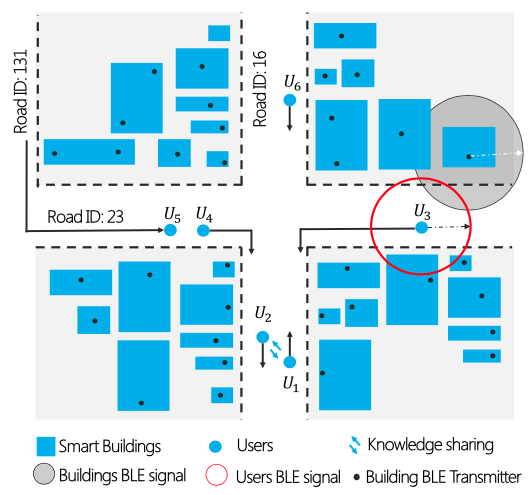
\includegraphics[width=0.5\textwidth]{smart_city}
\end{figure}

\begin{table}[h]
\caption{A simplified example of the SPOIs table, taken from \cite{SC}}
\label{table_1}
\centering
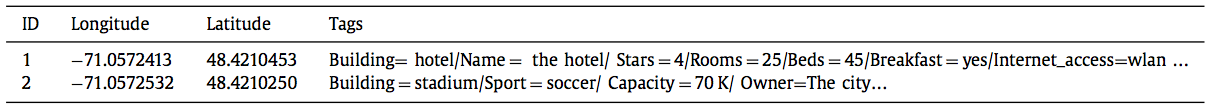
\includegraphics[width=0.5\textwidth]{table_1}
\end{table}

\begin{figure}[h]
\caption{An example of one user's Knowledge Circle, taken from \cite{SC}}
\label{kc}
\centering
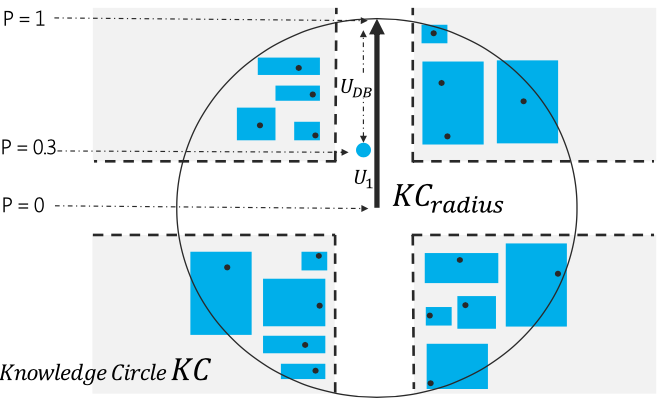
\includegraphics[width=0.5\textwidth]{KC}
\end{figure}

\begin{figure}[h]
\caption{Example of a user's knowledge with one global KC and two smaller KCs, taken from \cite{SC}}
\label{big_kc}
\centering
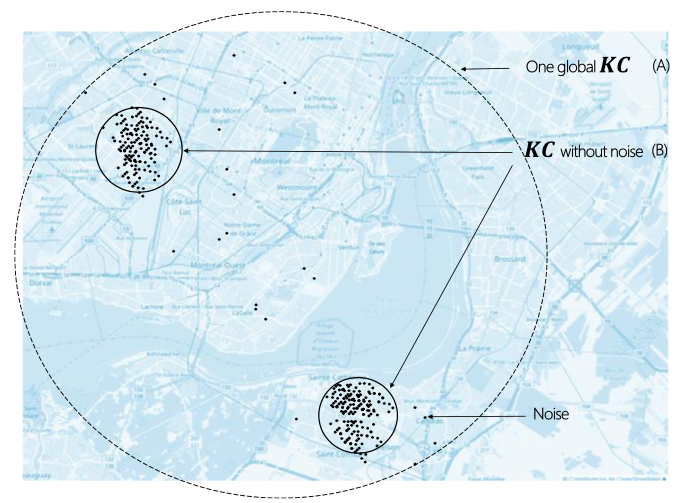
\includegraphics[width=0.5\textwidth]{big_kc}
\end{figure}

\begin{table}[h]
\caption{The variation of ESI (exploration satisfaction indicator) in function of the exploration radius, taken from \cite{SC}}
\label{table_2}
\centering
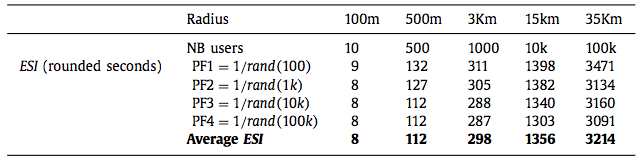
\includegraphics[width=0.5\textwidth]{esi_table}
\end{table}

\end{document}
